% Options for packages loaded elsewhere
\PassOptionsToPackage{unicode}{hyperref}
\PassOptionsToPackage{hyphens}{url}
%
\documentclass[
]{article}
\usepackage{lmodern}
\usepackage{amssymb,amsmath}
\usepackage{ifxetex,ifluatex}
\ifnum 0\ifxetex 1\fi\ifluatex 1\fi=0 % if pdftex
  \usepackage[T1]{fontenc}
  \usepackage[utf8]{inputenc}
  \usepackage{textcomp} % provide euro and other symbols
\else % if luatex or xetex
  \usepackage{unicode-math}
  \defaultfontfeatures{Scale=MatchLowercase}
  \defaultfontfeatures[\rmfamily]{Ligatures=TeX,Scale=1}
\fi
% Use upquote if available, for straight quotes in verbatim environments
\IfFileExists{upquote.sty}{\usepackage{upquote}}{}
\IfFileExists{microtype.sty}{% use microtype if available
  \usepackage[]{microtype}
  \UseMicrotypeSet[protrusion]{basicmath} % disable protrusion for tt fonts
}{}
\makeatletter
\@ifundefined{KOMAClassName}{% if non-KOMA class
  \IfFileExists{parskip.sty}{%
    \usepackage{parskip}
  }{% else
    \setlength{\parindent}{0pt}
    \setlength{\parskip}{6pt plus 2pt minus 1pt}}
}{% if KOMA class
  \KOMAoptions{parskip=half}}
\makeatother
\usepackage{xcolor}
\IfFileExists{xurl.sty}{\usepackage{xurl}}{} % add URL line breaks if available
\IfFileExists{bookmark.sty}{\usepackage{bookmark}}{\usepackage{hyperref}}
\hypersetup{
  pdftitle={ASSIGNMENT 4},
  pdfauthor={Michael Paris},
  hidelinks,
  pdfcreator={LaTeX via pandoc}}
\urlstyle{same} % disable monospaced font for URLs
\usepackage[margin=1in]{geometry}
\usepackage{graphicx,grffile}
\makeatletter
\def\maxwidth{\ifdim\Gin@nat@width>\linewidth\linewidth\else\Gin@nat@width\fi}
\def\maxheight{\ifdim\Gin@nat@height>\textheight\textheight\else\Gin@nat@height\fi}
\makeatother
% Scale images if necessary, so that they will not overflow the page
% margins by default, and it is still possible to overwrite the defaults
% using explicit options in \includegraphics[width, height, ...]{}
\setkeys{Gin}{width=\maxwidth,height=\maxheight,keepaspectratio}
% Set default figure placement to htbp
\makeatletter
\def\fps@figure{htbp}
\makeatother
\setlength{\emergencystretch}{3em} % prevent overfull lines
\providecommand{\tightlist}{%
  \setlength{\itemsep}{0pt}\setlength{\parskip}{0pt}}
\setcounter{secnumdepth}{-\maxdimen} % remove section numbering

\title{ASSIGNMENT 4}
\author{Michael Paris}
\date{2020-01-06}

\begin{document}
\maketitle

\hypertarget{markdown-basics}{%
\section{Markdown Basics}\label{markdown-basics}}

\hypertarget{favorite-foods}{%
\subsection{Favorite Foods}\label{favorite-foods}}

\begin{enumerate}
\def\labelenumi{\arabic{enumi}.}
\tightlist
\item
  Barbecue Brisket
\item
  Lasagna
\item
  Mexican (Any Mexican)
\end{enumerate}

\hypertarget{images}{%
\subsection{Images}\label{images}}

\begin{figure}
\centering
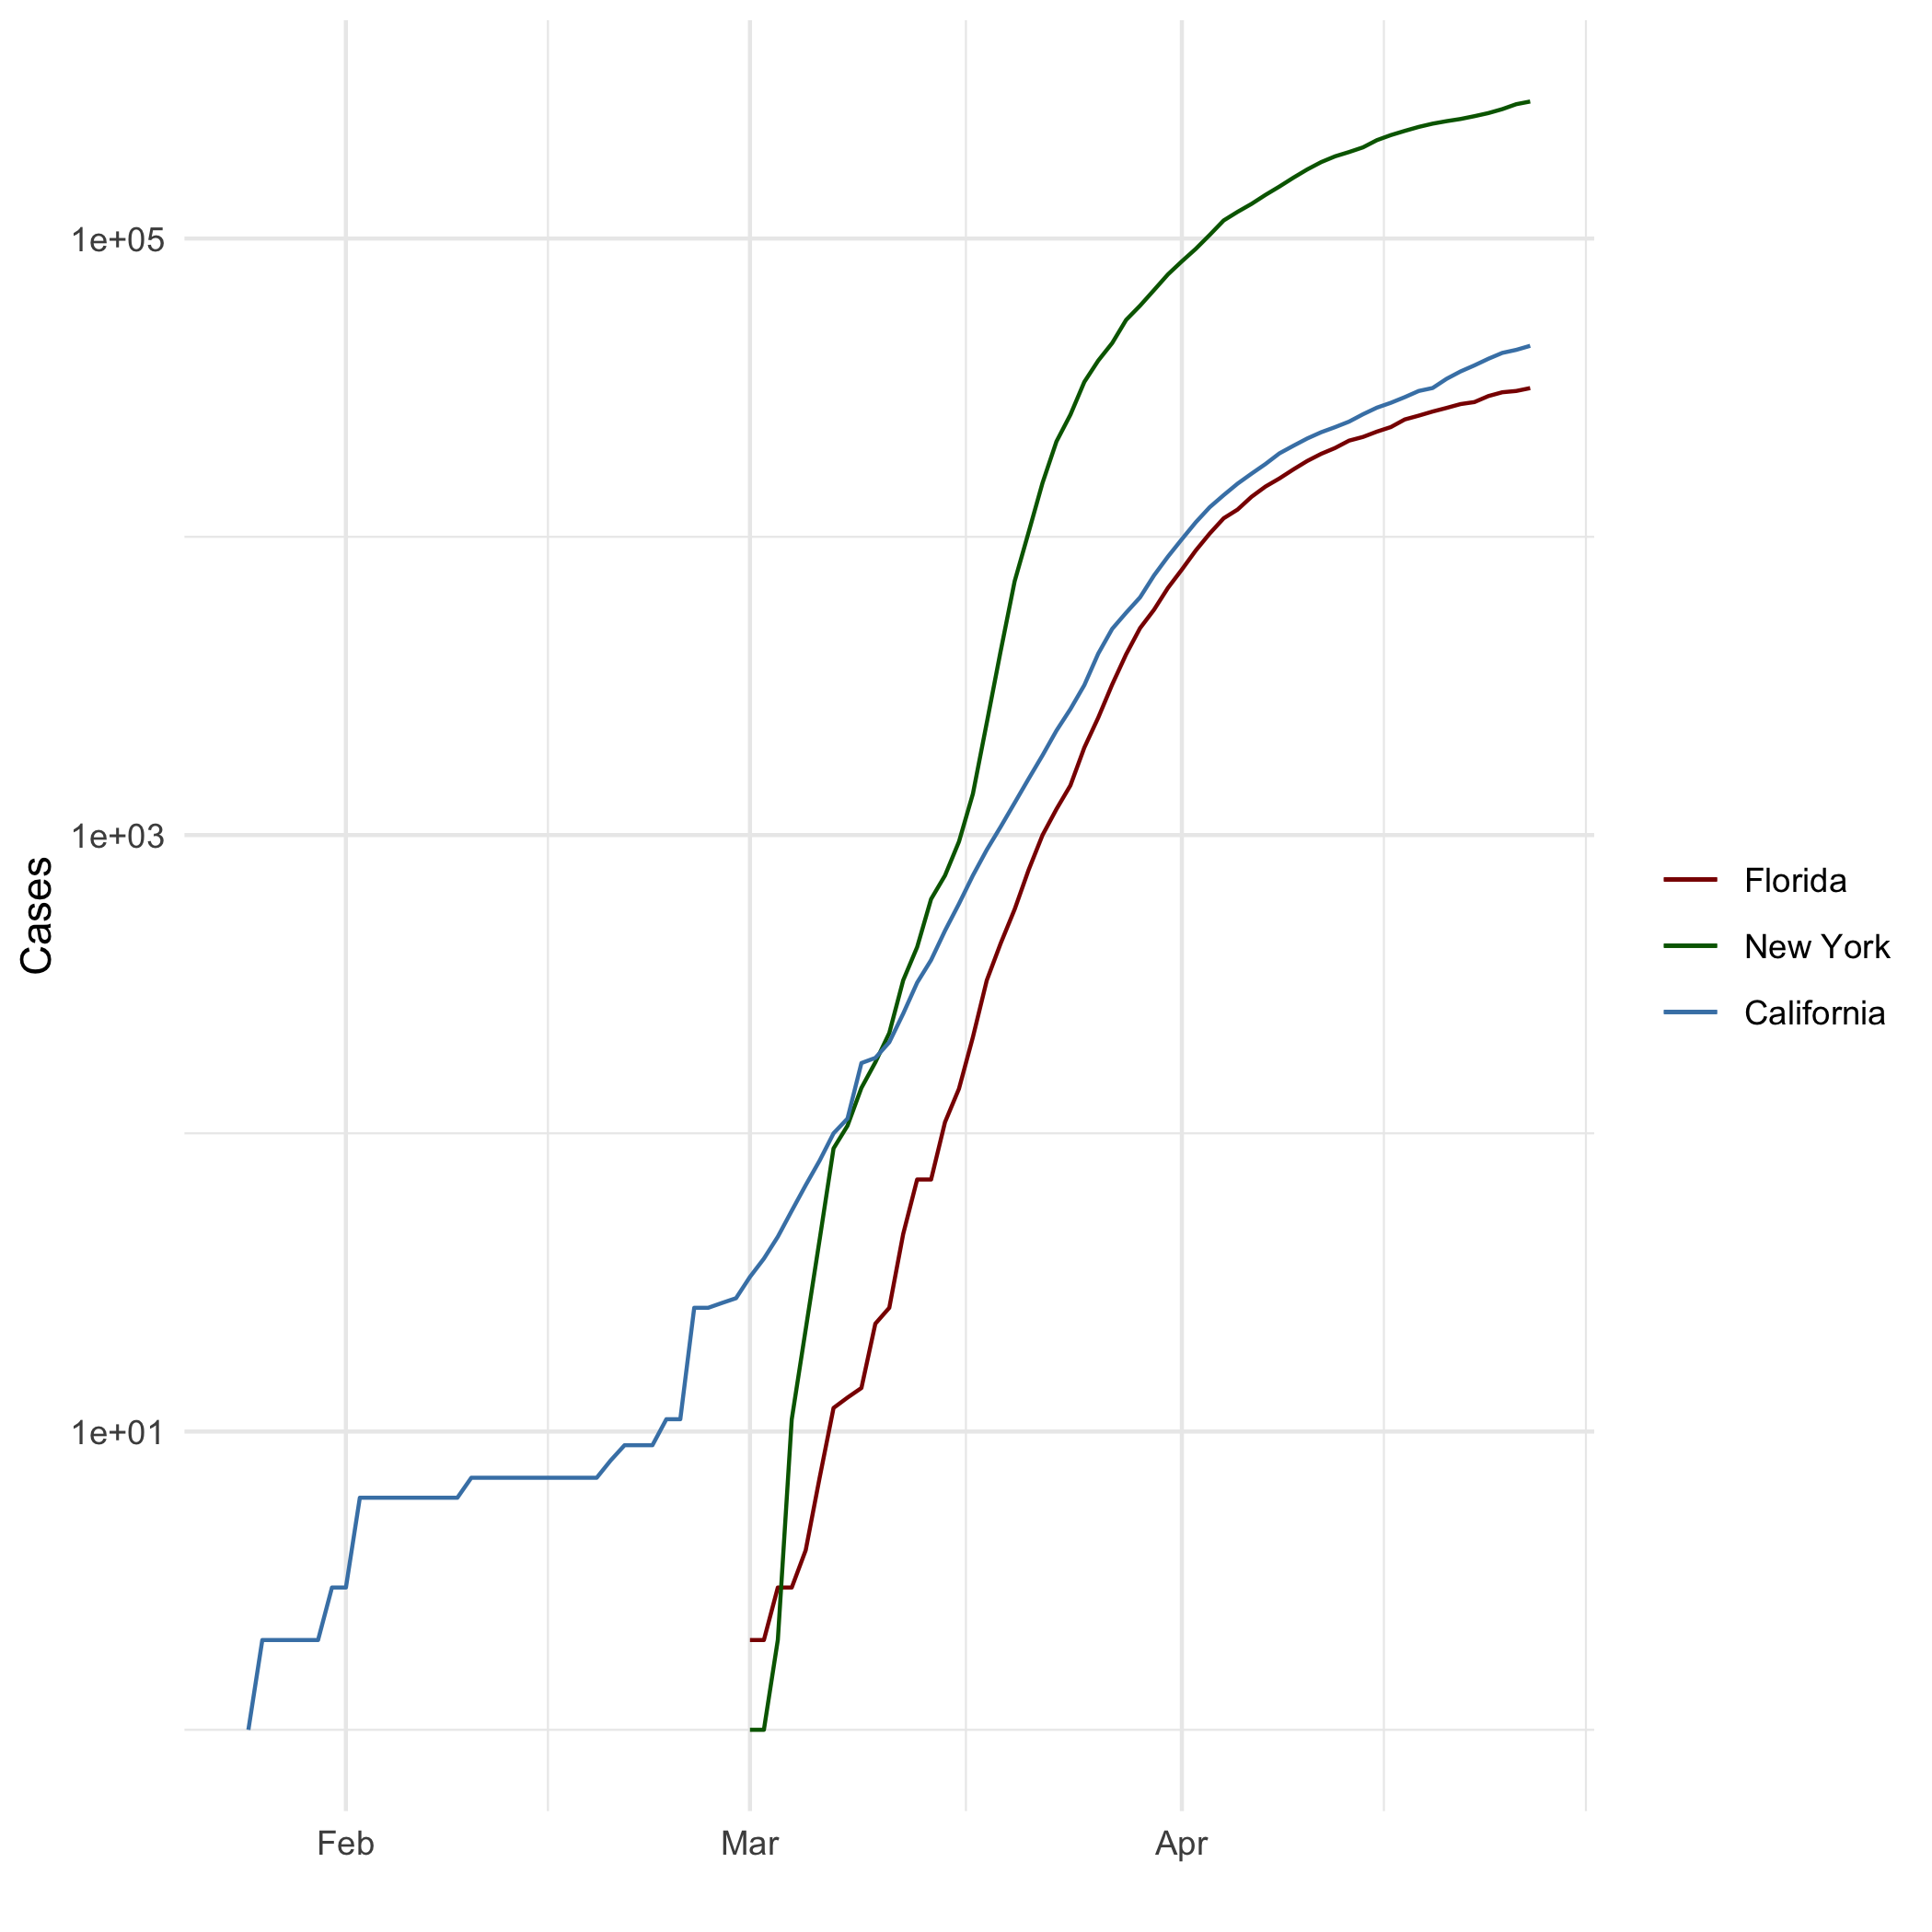
\includegraphics{plots/10-all-cases-log.png}
\caption{All Cases (Log Plot)}
\end{figure}

\hypertarget{add-a-quote}{%
\subsection{Add a Quote}\label{add-a-quote}}

\hypertarget{changed-this-to-favorite-movie-quote}{%
\subsection{Changed this to favorite movie
quote}\label{changed-this-to-favorite-movie-quote}}

\begin{quote}
As far back as I can remember, I always wanted to be a gangster.
\end{quote}

\hypertarget{add-an-equation}{%
\subsection{Add an Equation}\label{add-an-equation}}

\hypertarget{add-a-footnote}{%
\subsection{Add a Footnote}\label{add-a-footnote}}

This is a footnote

\hypertarget{add-citations}{%
\subsection{Add Citations}\label{add-citations}}

\begin{itemize}
\tightlist
\item
  R for Everyone
\item
  Discovering Statistics Using R
\end{itemize}

\hypertarget{inline-code}{%
\section{Inline Code}\label{inline-code}}

\hypertarget{ny-times-covid-19-data}{%
\subsection{NY Times COVID-19 Data}\label{ny-times-covid-19-data}}

\hypertarget{r4ds-height-vs-earnings}{%
\subsection{R4DS Height vs Earnings}\label{r4ds-height-vs-earnings}}

\hypertarget{tables}{%
\section{Tables}\label{tables}}

\hypertarget{knitr-table-with-kable}{%
\subsection{Knitr Table with Kable}\label{knitr-table-with-kable}}

\hypertarget{pandoc-table}{%
\subsection{Pandoc Table}\label{pandoc-table}}

\hypertarget{references}{%
\section{References}\label{references}}

\end{document}
